% !TeX program = pdflatex
% !TeX encoding = UTF-8
% !TeX spellcheck = it_IT

\documentclass[9pt]{beamer}

%********************************************************************
% Packages
%********************************************************************

\usepackage[utf8]{inputenc}
\usepackage[T1]{fontenc}
\usepackage[english]{babel}
\usepackage[bottom, para]{footmisc}
\usepackage{amsmath,amssymb,amsthm}
\usepackage{graphicx}
\usepackage{hyperref}
\usepackage{listings}
\usepackage{perpage}
\usepackage{xcolor}
\usepackage{wrapfig}
\usepackage{ifthen}
\usepackage{scrextend} % add margin to answers
\usepackage{dashrule}

%********************************************************************
% Packages options
%********************************************************************

% geometry
\usepackage{geometry}
\geometry{
    a4paper,
    ignoremp,
    bindingoffset = 1cm, 
    textwidth     = 13.5cm,
    textheight    = 21.5cm,
    lmargin       = 1cm,
    rmargin		    = 3cm,
    tmargin       = 2cm,
    bmargin       = 3cm
}

% listings
\renewcommand{\lstlistingname}{Code}

\definecolor{lightgray}{rgb}{.9,.9,.9}
\definecolor{darkgray}{rgb}{.4,.4,.4}
\definecolor{purple}{rgb}{0.65, 0.12, 0.82}
\lstset{
  basicstyle=\small\sffamily,
  numbers=left,
  numberstyle=\tiny,
  numbersep=3pt,
  stepnumber=1,
  frame=tb,
  columns=fullflexible,
  backgroundcolor=\color{yellow!15},
  keywordstyle=\color{blue}\bfseries,
  ndkeywordstyle=\color{darkgray}\bfseries,
  identifierstyle=\color{black},
  commentstyle=\color{purple}\ttfamily,
  stringstyle=\color{red}\ttfamily,
  numberbychapter=false,
  showstringspaces=false,
  breaklines=true,
  captionpos=b, % put captions at the bottom 
}
%\lstset{
%  numbersep=5pt,
%  frame=trbl
%}

\definecolor{prismgreen}{rgb}{0.12, 0.48, 0.12}
\lstdefinelanguage{prism}{ % syntax highlight via font
  keywords={
    bool,C,ceil,const,ctmc,double,dtmc,endinit,endmodule,endrewards,endsystem,F,false,floor,formula,G,global,I,init,int,label,max,mdp,min,module,nondeterministic,P,Pmin,Pmax,prob,probabilistic,R,rate,rewards,Rmin,Rmax,S,stochastic,system,true,U,X
  }, 
  keywordstyle={\bfseries\color{black}}, 
  numberstyle=\tiny\color{black}, 
  comment=[l] {//}, morecomment=[s]{/*}{*/}, % single and multi-line 
  commentstyle= \color{prismgreen}, % dark green 
  tabsize=4, % tab treatment (going to be fixed in Prism)
  escapechar=@ % write LaTeX comments escaped by @ symbol 
} 

% perpage
\MakePerPage{footnote}

% hyperref
\definecolor{webgreen}{rgb}{0,.5,0}
\definecolor{webbrown}{rgb}{.6,0,0}
\definecolor{RoyalBlue}{cmyk}{1, 0.50, 0, 0}
\hypersetup{%
  %draft, % = no hyperlinking at all (useful in b/w printouts)
  colorlinks=true, linktocpage=true, pdfstartpage=3, pdfstartview=FitV,%
  % uncomment the following line if you want to have black links (e.g., for printing)
  % colorlinks=false, linktocpage=false, pdfstartpage=3, pdfstartview=FitV, pdfborder={0 0 0},%
  breaklinks=true, pdfpagemode=UseNone, pageanchor=true, pdfpagemode=UseOutlines,%
  plainpages=false, bookmarksnumbered, bookmarksopen=true, bookmarksopenlevel=1,%
  hypertexnames=true, pdfhighlight=/O,%nesting=true,%frenchlinks,%
  urlcolor=RoyalBlue, linkcolor=black, citecolor=webbrown, %pagecolor=RoyalBlue,%
  %urlcolor=Black, linkcolor=Black, citecolor=Black, %pagecolor=Black,%
}

% graphicx
\graphicspath{{img/}}

%********************************************************************
% New commands
%********************************************************************

\newcommand{\question}[1]{%
  \vspace{20pt}%
  \begin{wrapfigure}{l}{0.1\textwidth}%
    \vspace{-30pt}%
    \begin{center}%
      
\includegraphics[scale=1]{hand.jpg}%
    \end{center}%
    \vspace{-30pt}%
  \end{wrapfigure}%
  \noindent #1%
}%
\newcommand{\answer}[1]{%
  \vspace{5pt}\par\noindent
  \textbf{\underline{Answer:}}%
  \begin{addmargin}[1em]{1em}% 1em left, 2em right
    #1%
    \begin{flushright}%
      \qedsymbol%
    \end{flushright}%
  \end{addmargin}%
}%

\definecolor{light-gray}{gray}{0.95}
\newboolean{inlineCodeBackground}
\setboolean{inlineCodeBackground}{false}
\newcommand{\prism}[1]{%
  \ifthenelse{\boolean{inlineCodeBackground}}{%
    \colorbox{light-gray}{\lstinline[language=prism]{#1}}%
  }{%
    \lstinline[language=prism]{#1}%
  }%
}%
\newcommand{\bash}[1]{%
  \ifthenelse{\boolean{inlineCodeBackground}}{%
    \colorbox{light-gray}{\lstinline[language=bash]{#1}}%
  }{%
    \lstinline[language=bash]{#1}%
  }%
}%

\newcommand{\dashedrule}{%
  \noindent\hdashrule{\textwidth}{1pt}{1.5mm}%
}%


\title[Riordino intelligente tramite MDP]{Riordino intelligente dei farmaci tramite modelli MDP}
\author{M.Biagi \and \textbf{T.Papini} \and}
\institute{
    STLab, Dipartimento d'Ingegneria dell'Informazione, Università degli Studi di Firenze, Italia,\\
    {\{marco.biagi,tommaso.papini\}@unifi.it}
}
\date{31 Marzo 2017}

\begin{document}

    \begin{frame}
        \titlepage
        \begin{itemize}
            \item Tecniche basate su MDP
            \begin{itemize}
                \item modellazione del reparto
                \item attualizzazione del modello
                \item sperimentazione
            \end{itemize}
        \end{itemize}
    \end{frame}

    \begin{frame}{Panoramica}
        %\tiny
        \tableofcontents
    \end{frame}

    \section{Il modello generale}
    
        \subsection{Struttura del modello}
            \begin{frame}{Struttura del modello}
              \begin{itemize}
                \item Modellazione di più giorni consecutivi
                \begin{itemize}
                  \item giorno corrente (fine giornata)
                  \item 3 giorni successivi
                \end{itemize}
                \item probabilità e non-determinismo
                \begin{itemize}
                  \item evoluzione probabilistica di ogni giornata
                  \item scelte non-deterministiche sull'ordine
                \end{itemize}
              \end{itemize}
              \vspace{1cm}
              \begin{center}
                \begin{tikzpicture}[node distance = 2cm, auto]
                  % Place nodes
                  \node [block, circle] at (0,0) (oggi) [] {Giorno\\corrente};
                  \node [block, circle] at (2.5,0) (g1) [] {Giorno 1};
                  \node [block, circle] at (5,0) (g2) [] {Giorno 2};
                  \node [block, circle] at (7.5,0) (g3) [] {Giorno 3};
                  % Draw edges
                  \path [line] (oggi) to [out=40,in=140] (g1);
                  \path [line] (oggi) -- (g1);
                  \path [line] (oggi) to [out=-40,in=-140] (g1);
                  
                  \path [line] (g1) to [out=40,in=140] (g2);
                  \path [line] (g1) -- (g2);
                  \path [line] (g1) to [out=-40,in=-140] (g2);
                  
                  \path [line] (g2) to [out=40,in=140] (g3);
                  \path [line] (g2) -- (g3);
                  \path [line] (g2) to [out=-40,in=-140] (g3);
                \end{tikzpicture}
              \end{center}
              % schema con quantità dell'ordine
%              \begin{center}
%                \begin{tikzpicture}[node distance = 2cm, auto]
%                  % Place nodes
%                  \node [block] at (0,0) (oggi) [] {Giorno\\corrente};
%                  \node [block] at (2.5,0) (g1) [] {Giorno 1};
%                  \node [block] at (5,0) (g2) [] {Giorno 2};
%                  \node [block] at (7.5,0) (g3) [] {Giorno 3};
%                  % Draw edges
%                  \path [line] (oggi) to [out=40,in=140] node {0} (g1);
%                  \path [line] (oggi) -- node {10} (g1);
%                  \path [line] (oggi) to [out=-40,in=-140] node {20} (g1);
%                  
%                  \path [line] (g1) to [out=40,in=140] node {0} (g2);
%                  \path [line] (g1) -- node {10} (g2);
%                  \path [line] (g1) to [out=-40,in=-140] node {20} (g2);
%                  
%                  \path [line] (g2) to [out=40,in=140] node {0} (g3);
%                  \path [line] (g2) -- node {10} (g3);
%                  \path [line] (g2) to [out=-40,in=-140] node {20} (g3);
%                \end{tikzpicture}
%              \end{center}
            \end{frame}
        
        \subsection{Specifiche e limitazioni}
            \begin{frame}{Specifiche e limitazioni}
              \begin{itemize}
                \item Reparto
                \begin{itemize}
                  \item un reparto con posologia fissa
                  \item capienza del reparto fissata
                  \item capienza del magazzino fissata
                \end{itemize}
                \item Farmaco
                \begin{itemize}
                  \item un solo tipo di farmaco
                \end{itemize}
                \item Caratterizzazione probabilistica
                \begin{itemize}
                  \item pazienti in arrivo (programmati/pronto soccorso)
                  \item pazienti in uscita
                  \item consumo di farmaci per i pazienti in reparto
                \end{itemize}
                \item Scelte non-deterministiche
                \begin{itemize}
                  \item se e in che quantità riordinare $\{0,10,20,30,40\}$
                \end{itemize}
                \item Funzione di costo
                \begin{itemize}
                  \item costo dell'ordine di ogni unità di farmaco
                  \item costo della giacenza di ogni farmaco in magazzino
                  \item costo di farmaci mancanti da somministrare
                \end{itemize}
              \end{itemize}
            \end{frame}
            
    \section{Utilizzo del modello}
    
        \subsection{Strumenti utilizzati}
            \begin{frame}{Strumenti utilizzati}
              \begin{itemize}
                \item Componente Java
                \begin{itemize}
                  \item simulazione
                  \item attualizzazione
                  \item estrazione dell'avversario
                  \item sperimentazione
                \end{itemize}
                \vspace{0.8cm}
                \item Prism
                \begin{itemize}
                  \item Implementazione del modello attualizzato
                  \item Calcolo della strategia ottima
                \end{itemize}
              \end{itemize}
            \end{frame}
    
        \subsection{Calcolo della strategia ottima}
            \begin{frame}{Calcolo della strategia ottima}
              Ogni giorno, il modello viene attualizzato sulla base dei dati attuali.
              \begin{itemize}
                \item \textbf{Simulatore}: genera dati verosimili e consistenti
                \begin{itemize}
                  \item implementa le stesse distribuzioni di probabilità definite nel modello Prism
                \end{itemize}
                \item \textbf{Template}: rappresenta un generico modello Prism non attualizzato
                \begin{itemize}
                  \item attualizzato tramite il template engine Apache Velocity
                \end{itemize}
              \end{itemize}
              \vspace{1cm}
              Sul modello attualizzato, Prism può calcolare la strategia ottima
              \begin{itemize}
                \item Da componente Java
                \begin{itemize}
                  \item viene estratto l'avversario
                  \item che indica la scelta ottima
                \end{itemize}
              \end{itemize}
              \vspace{1cm}
              La scelta ottima suggerita da Prism \textbf{minimizza} il costo \textbf{medio} sui 3 giorni successivi! 
            \end{frame}
            
    \section{Sperimentazione}
    
        \begin{frame}{Sperimentazione}
          \begin{center}
            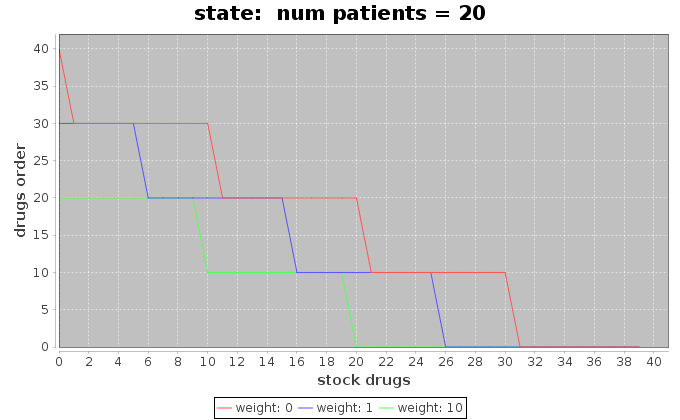
\includegraphics[scale=0.4]{test1.png}
          \end{center}
        \end{frame}

\end{document}
